\documentclass[preprint]{sigplanconf}

\usepackage{ifthen}
\usepackage{fancyvrb}
\usepackage{color}
\usepackage{ulem}
\usepackage{xspace}
\usepackage{epsfig}
\usepackage{amssymb}
\usepackage{amsmath}
\usepackage{amsfonts}
\usepackage[utf8]{inputenc}
\usepackage{setspace}

\usepackage{listings}

\usepackage[T1]{fontenc}
\usepackage{beramono}


\definecolor{gray}{rgb}{0.3,0.3,0.3}

\lstset{
  basicstyle=\setstretch{1.1}\ttfamily\footnotesize,
  language=Python,
  keywordstyle=\bfseries,
  stringstyle=\color{blue},
  commentstyle=\color{gray}\textit,
  fancyvrb=true,
  showstringspaces=false,
  %keywords={def,while,if,elif,return,class,get,set,new,guard_class}
  numberstyle = \tiny,
  numbersep = 0pt,
}


\newboolean{showcomments}
\setboolean{showcomments}{true}
\ifthenelse{\boolean{showcomments}}
  {\newcommand{\nb}[2]{
    \fbox{\bfseries\sffamily\scriptsize#1}
    {\sf\small$\blacktriangleright$\textit{#2}$\blacktriangleleft$}
   }
   \newcommand{\version}{\emph{\scriptsize$-$Id: main.tex 19055 2008-06-05 11:20:31Z cfbolz $-$}}
  }
  {\newcommand{\nb}[2]{}
   \newcommand{\version}{}
  }

\newcommand\cfbolz[1]{\nb{CFB}{#1}}
\newcommand\arigo[1]{\nb{AR}{#1}}
\newcommand\fijal[1]{\nb{FIJAL}{#1}}
\newcommand\david[1]{\nb{DAVID}{#1}}
\newcommand\anto[1]{\nb{ANTO}{#1}}
\newcommand\reva[1]{\nb{Reviewer 1}{#1}}
\newcommand\revb[1]{\nb{Reviewer 2}{#1}}
\newcommand\revc[1]{\nb{Reviewer 3}{#1}}
\newcommand{\commentout}[1]{}
\newcommand{\ignore}[1]{} % {{\tt \small ignore(#1)}}

\newcommand\ie{i.e.,\xspace}
\newcommand\eg{e.g.,\xspace}
\newcommand{\etal}{\emph{et al.}\xspace}

\normalem

\let\oldcite=\cite

\renewcommand\cite[1]{\ifthenelse{\equal{#1}{XXX}}{[citation~needed]}{\oldcite{#1}}}

%
\def\sharedaffiliation{%
\end{tabular}
\begin{tabular}{c}}
%
\begin{document}
\conferenceinfo{PEPM}{'11, Austin, USA}
\CopyrightYear{2011}
\copyrightdata{[to be supplied]}

\title{Allocation Removal by Partial Evaluation in a Tracing JIT}

\authorinfo{Carl Friedrich Bolz$^a$ \and Antonio Cuni$^a$ \and Maciej Fijałkowski$^b$ \and Michael Leuschel$^a$ \and \\
            Samuele Pedroni$^c$ \and Armin Rigo$^a$}
           {$^a$Heinrich-Heine-Universität Düsseldorf, STUPS Group, Germany

            $^b$merlinux GmbH, Hildesheim, Germany

            $^c$Open End, Göteborg, Sweden
           }
           {cfbolz@gmx.de \and anto.cuni@gmail.com \and fijal@merlinux.eu \and
           leuschel@cs.uni-duesseldorf.de \and samuele.pedroni@gmail.com \and arigo@tunes.org}

%\numberofauthors{3}
%\author{
%\alignauthor Carl Friedrich Bolz\\
%       \email{cfbolz@gmx.de}
%\alignauthor Michael Leuschel\\
%       \email{leuschel@cs.uni-duesseldorf.de}
%\alignauthor David Schneider\\
%      \email{david.schneider@uni-duesseldorf.de}
%      \sharedaffiliation
%      \affaddr{Heinrich-Heine-Universität Düsseldorf, STUPS Group, Germany}\\
%}

\maketitle
\begin{abstract}
The performance of many dynamic language implementations suffers from
high allocation rates and runtime type checks.  This makes dynamic
languages less applicable to purely algorithmic problems, despite their
growing popularity.  In this paper we present a simple compiler optimization
based on online partial evaluation to remove object allocations and
runtime type checks in the context of a tracing JIT.  We evaluate the
optimization using a Python VM and find that it gives good results for
all our (real-life) benchmarks.
\footnote{This research is partially supported by the BMBF funded project PyJIT (nr. 01QE0913B;
Eureka Eurostars).}
\end{abstract}

% A category with the (minimum) three required fields
%\category{H.4}{Information Systems Applications}{Miscellaneous}
%A category including the fourth, optional field follows...
%\category{D.2.8}{Software Engineering}{Metrics}[complexity measures, performance measures]

\category{D.3.4}{Programming Languages}{Processors}[code generation,
interpreters, run-time environments]

\terms
Languages, Performance, Experimentation

\keywords{Tracing JIT, Partial Evaluation, Optimization}

\section{Introduction}

The objective of a just-in-time (JIT) compiler for a dynamic language is to
improve the speed of the language over an implementation of the language that
uses interpretation. The first goal of a JIT is therefore to remove the
interpretation overhead, i.e. the overhead of bytecode (or AST) dispatch and the
overhead of the interpreter's data structures, such as operand stack etc. The
second important problem that any JIT for a dynamic language needs to solve is
how to deal with the overhead of boxing primitive types and of type
dispatching. Those are problems that are usually not present or at least less
severe in statically typed languages.

Boxing of primitive types is necessary because dynamic languages need to be able to handle
all objects, even integers, floats, booleans etc. in the same way as user-defined
instances. Thus those primitive types are usually \emph{boxed}, \ie a small
heap-structure is allocated for them that contains the actual value. Boxing
primitive types can be very costly, because a lot of common operations,
particularly all arithmetic operations, have to produce new boxes, in addition
to the actual computation they do. Because the boxes are allocated on the heap,
producing many of them puts pressure on the garbage collector.

Type dispatching is the process of finding the concrete implementation that is
applicable to the objects at hand when performing a generic operation on them. An
example would be the addition of two objects: For addition the types of the
concrete objects need to be checked and the suiting implementation chosen.
Type dispatching is a very common operation in
modern\footnote{For languages in the LISP family, basic arithmetic operations
are typically not overloaded; even in Smalltalk, type dispatching is much
simpler than in Python or JavaScript.}
dynamic languages because no types are known at compile time. Therefore all
operations need it.

A recently popular approach to implementing just-in-time compilers for dynamic
languages is that of a tracing JIT. A tracing JIT works by observing the running
program and recording its hot spots into \emph{linear execution traces}. Those
traces are optimized and turned into machine code.

One reason for the popularity of tracing JITs is their relative
simplicity. They can often be added to an existing interpreter, reusing a lot of
the interpreter's infrastructure. They give some important
optimizations like inlining and constant-folding for free. A tracing JIT always
produces linear pieces of code, which simplifies many of the hard algorithms in
a compiler, such as register allocation.

The use of a tracing JIT can remove the overhead of bytecode dispatch and that
of the interpreter data structures. In this paper we want to present a new
optimization that can be added to a tracing JIT that further removes some of the
overhead more closely associated to dynamic languages, such as boxing overhead
and type dispatching. Our experimental platform is the PyPy project, which is an
environment for implementing dynamic programming languages. PyPy and tracing
JITs are described in more detail in Section~\ref{sec:Background}.
Section~\ref{sec:lifetimes} analyzes the problem to be solved more closely.

The core of our trace optimization technique can be
viewed as partial evaluation: the partial evaluation
performs a form of escape analysis \cite{bruno_blanchet_escape_2003} on the traces and makes some
objects that are allocated in the trace \emph{static,} which
means that they do not occur any more in the optimized trace. This technique is
informally described in Section~\ref{sec:statics}; a more formal description is
given in Section~\ref{sec:formal}. The introduced
techniques are evaluated in Section~\ref{sec:Evaluation} using PyPy's Python
interpreter.

The contributions made by this paper are:

\begin{enumerate}
    \item A description of an efficient and effective algorithm for removing
          object allocations in a tracing JIT.
    \item A characterization of this algorithm as partial evaluation.
    \item Performance benchmarks for this algorithm.
\end{enumerate}


\section{Background}
\label{sec:Background}

\subsection{PyPy}
\label{sub:PyPy}

The work described in this paper was done in the context of the PyPy project\footnote{\texttt{http://pypy.org}}
\cite{armin_rigo_pypys_2006}. PyPy is an environment where dynamic languages can
be implemented in a simple yet efficient way. 
When implementing a language with PyPy one writes an \emph{interpreter}
for the language in
\emph{RPython} \cite{davide_ancona_rpython:_2007}. RPython ("restricted Python")
is a subset of Python chosen in such a way that type inference becomes
possible. The language interpreter can then be compiled (``translated'') with
PyPy's tools into a VM on C level. During translation to C, many low-level
aspects of the final VM, such as object layout, garbage collection and memory
model, are woven into the generated code. Therefore the interpreter itself can
remain at a relatively high level of abstraction.

A number of languages have been implemented with PyPy. The project was initiated
to get a better Python implementation, which inspired the name of the project
and is still the main focus of development. In addition a number of other
languages were implemented, among them a Prolog interpreter
\cite{carl_friedrich_bolz_towards_2010}, a Smalltalk VM
\cite{carl_friedrich_bolz_back_2008} and a GameBoy emulator
\cite{bruni_pygirl:_2009}.

The feature that makes PyPy more than a compiler with a runtime system is its
support for automated JIT compiler generation \cite{bolz_tracing_2009}. During
the translation to C, PyPy's tools can generate a tracing just-in-time compiler for the
language that the interpreter is implementing. This process is mostly
automatic; it only needs to be guided by the language implementer using a small number of
source-code hints. Mostly-automatically generating a JIT compiler has many advantages
over writing one manually, an error-prone and tedious process.
By construction, the generated JIT has the same semantics as the interpreter.
Optimizations can be shared between different languages implemented with PyPy.

Moreover, thanks to the internal design of the JIT generator, it is very easy
to add new \emph{backends} for producing the actual machine code.  Examples of
JIT backends that are implemented are those for Intel x86 and x86-64 and an
experimental one for the CLI .NET Virtual Machine \cite{cuni_high_2010}.

\subsection{Tracing JIT Compilers}
\label{sub:JIT_background}

Tracing JITs are a recently popular approach to write just-in-time compilers for
dynamic languages. Their origins lie in the Dynamo project, which used a tracing
approach to optimize machine code using execution traces
\cite{bala_dynamo:_2000}. Tracing JITs have then be adapted to be used for a
very light-weight Java VM \cite{gal_hotpathvm:_2006} and afterwards used in
several implementations of dynamic languages, such as JavaScript
\cite{andreas_gal_trace-based_2009}, Lua\footnote{\texttt{http://luajit.org/}}
and now Python (and other languages) via PyPy.

The core idea of tracing JITs is to focus the optimization effort of the JIT
compiler on the commonly executed, \ie \emph{hot} paths of the core loops of the program and to just use an
interpreter for the less commonly executed parts. VMs that use a tracing JIT are
mostly mixed-mode execution environments, they contain both an interpreter and a
JIT compiler. By default the interpreter is used to execute the program, doing
some light-weight profiling at the same time. This profiling is used to identify
the hot loops of the program. If a hot loop is found in that way, the
interpreter enters a special \emph{tracing mode}. In this tracing mode, the
interpreter tries to record all operations that it is executing while running one
iteration of the hot loop. This history of executed operations of one loop is
called a \emph{trace}. Because the trace corresponds to one iteration of a loop,
it always ends with a jump to its own beginning. The trace also contains all
operations that are performed in functions that were called in the loop, thus a
tracing JIT automatically performs inlining.
This trace of operations subsequently forms the basis of the generated code. The trace is
first optimized, and then turned into machine code. Both optimization
and machine code generation are simple, because the traces are linear. This
linearity makes many optimizations a lot more tractable, and the inlining that
happens gives the optimizations automatically more context to work with.

Since the trace corresponds to one concrete execution of a loop,
the code generated from it is only one possible path through the loop.
To make sure that the trace maintains the correct semantics, it contains a
\emph{guard} at all places where the execution could have diverged from the
path. Those guards check the assumptions under which execution can stay on the
trace. As an example, if a loop contains an if-statement, the trace
will contain the execution of one of the paths only, which is the path that was
taken during the production of the trace. The trace will also contain a guard
that checks that the condition of the if-statement is the same as
during tracing, because if
it isn't, the rest of the trace would not be valid.

When generating machine code, every guard is be turned into a quick check to
see whether the assumption still holds. When such a guard is hit during the
execution of the machine code and the assumption does not hold, the execution of
the machine code is stopped, and interpreter continues to run from that point
on. These guards are the only mechanism to stop the execution of a trace, the
loop end condition also takes the form of a guard.

If one specific guard fails often enough, the tracing JIT will generate a new
trace that starts exactly at the position of the failing guard. The existing
assembler is patched to jump to the new trace when the guard fails
\cite{andreas_gal_incremental_2006}.  This approach guarantees that all the
hot paths in the program will eventually be traced and compiled into efficient
code.

\subsection{Running Example}
\label{sub:example}

For the purpose of this paper, we are going to use a tiny interpreter for a dynamic language with
 a very simple object
model, that just supports an integer and a float type. The objects support only
two operations, \lstinline{add}, which adds two objects (promoting ints to floats in a
mixed addition) and \lstinline{is_positive}, which returns whether the number is greater
than zero. The implementation of \lstinline{add} uses classical Smalltalk-like
double-dispatching.
%These classes could be part of the implementation of a very
%simple interpreter written in RPython.
The classes can be seen in
Figure~\ref{fig:objmodel} (written in RPython).

\begin{figure}
\begin{lstlisting}[mathescape]
class Base(object):
   pass

class BoxedInteger(Base):
   def __init__(self, intval):
      self.intval = intval

   def add(self, other):
      return other.add__int(self.intval)

   def add__int(self, intother):
      return BoxedInteger(intother + self.intval)

   def add__float(self, floatother):
      floatvalue = floatother + float(self.intval)
      return BoxedFloat(floatvalue)

   def is_positive(self):
      return self.intval > 0

class BoxedFloat(Base):
   def __init__(self, floatval):
      self.floatval = floatval

   def add(self, other):
      return other.add__float(self.floatval)

   def add__int(self, intother):
      floatvalue = float(intother) + self.floatval
      return BoxedFloat(floatvalue)

   def add__float(self, floatother):
      return BoxedFloat(floatother + self.floatval)

   def is_positive(self):
      return self.floatval > 0.0


def f(y):
   res = BoxedInteger(0)
   while y.is_positive():
      res = res.add(y).add(BoxedInteger(-100))
      y = y.add(BoxedInteger(-1))
   return res
\end{lstlisting}
\caption{An ``Interpreter'' for a Tiny Dynamic Language Written in RPython}
\label{fig:objmodel}
\end{figure}

Using these classes to implement arithmetic shows the basic problem of a
dynamic language implementation. All the numbers are instances of either
\lstinline{BoxedInteger} or \lstinline{BoxedFloat}, therefore they consume space on the
heap. Performing many arithmetic operations produces lots of garbage quickly,
putthing pressure on the garbage collector. Using double dispatching to
implement the numeric tower needs two method calls per arithmetic operation,
which is costly due to the method dispatch.

Let us now consider a simple interpreter function \lstinline{f} that uses the
object model (see the bottom of Figure~\ref{fig:objmodel}).
The loop in \lstinline{f} iterates \lstinline{y} times, and computes something in the process.
Simply running this function is slow, because there are lots of virtual method
calls inside the loop, one for each \lstinline{is_positive} and even two for each
call to \lstinline{add}. These method calls need to check the type of the involved
objects repeatedly and redundantly. In addition, a lot of objects are created
when executing that loop, many of these objects are short-lived.
The actual computation that is performed by \lstinline{f} is simply a sequence of
float or integer additions.


\begin{figure}
\begin{lstlisting}[mathescape,numbers = right]
# arguments to the trace: $p_{0}$, $p_{1}$
# inside f: res.add(y)
guard_class($p_{1}$, BoxedInteger)
    # inside BoxedInteger.add
    $i_{2}$ = get($p_{1}$, intval)
    guard_class($p_{0}$, BoxedInteger)
        # inside BoxedInteger.add__int
        $i_{3}$ = get($p_{0}$, intval)
        $i_{4}$ = int_add($i_{2}$, $i_{3}$)
        $p_{5}$ = new(BoxedInteger)
            # inside BoxedInteger.__init__
            set($p_{5}$, intval, $i_{4}$)

# inside f: BoxedInteger(-100) 
$p_{6}$ = new(BoxedInteger)
    # inside BoxedInteger.__init__
    set($p_{6}$, intval, -100)

# inside f: .add(BoxedInteger(-100))
guard_class($p_{5}$, BoxedInteger)
    # inside BoxedInteger.add
    $i_{7}$ = get($p_{5}$, intval)
    guard_class($p_{6}$, BoxedInteger)
        # inside BoxedInteger.add__int
        $i_{8}$ = get($p_{6}$, intval)
        $i_{9}$ = int_add($i_{7}$, $i_{8}$)
        $p_{10}$ = new(BoxedInteger)
            # inside BoxedInteger.__init__
            set($p_{10}$, intval, $i_{9}$)

# inside f: BoxedInteger(-1)
$p_{11}$ = new(BoxedInteger)
    # inside BoxedInteger.__init__
    set($p_{11}$, intval, -1)

# inside f: y.add(BoxedInteger(-1))
guard_class($p_{0}$, BoxedInteger)
    # inside BoxedInteger.add
    $i_{12}$ = get($p_{0}$, intval)
    guard_class($p_{11}$, BoxedInteger)
        # inside BoxedInteger.add__int
        $i_{13}$ = get($p_{11}$, intval)
        $i_{14}$ = int_add($i_{12}$, $i_{13}$)
        $p_{15}$ = new(BoxedInteger)
            # inside BoxedInteger.__init__
            set($p_{15}$, intval, $i_{14}$)

# inside f: y.is_positive()
guard_class($p_{15}$, BoxedInteger)
    # inside BoxedInteger.is_positive
    $i_{16}$ = get($p_{15}$, intval)
    $i_{17}$ = int_gt($i_{16}$, 0)
# inside f
guard_true($i_{17}$)
jump($p_{15}$, $p_{10}$)
\end{lstlisting}
\caption{An Unoptimized Trace of the Example Interpreter}
\label{fig:unopt-trace}
\end{figure}

If the function is executed using the tracing JIT, with \lstinline{y} being a
\lstinline{BoxedInteger}, the produced trace looks like the one of
Figure~\ref{fig:unopt-trace} (lines starting with a hash ``\#'' are comments).
The trace corresponds to one iteration of the while-loop in \lstinline{f}.

The operations in the trace are indented
corresponding to the stack level of the function that contains the traced
operation. The trace is in single-assignment form, meaning that each variable is
assigned a value exactly once. The arguments $p_0$ and $p_1$ of the loop correspond
to the live variables \lstinline{y} and \lstinline{res} in the original function.

The operations in the trace correspond to the operations in the RPython program
in Figure~\ref{fig:objmodel}:

\begin{itemize}
    \item \lstinline{new} creates a new object.
    \item \lstinline{get} reads an attribute of an object.
    \item \lstinline{set} writes to an attribute of an object.
    \item \lstinline{guard_class} is a precise type check and precedes an
    (inlined) method call and is followed by the trace of the called method.
    \item \lstinline{int_add} and \lstinline{int_gt} are integer addition and
    comparison (``greater than''), respectively.
\end{itemize}

The method calls in the trace are always preceded by a \lstinline{guard_class}
operation, to check that the class of the receiver is the same as the one that
was observed during tracing.\footnote{\lstinline{guard_class} performs a precise
class check, not checking for subclasses.} These guards make the trace specific
to the situation where \lstinline{y} is really a \lstinline{BoxedInteger}. When
the trace is turned into machine code and afterwards executed with
\lstinline{BoxedFloat}, the
first \lstinline{guard_class} instruction will fail and execution will continue
using the interpreter.

The trace shows the inefficiencies of \lstinline{f} clearly, if one looks at
the number of \lstinline{new}, \lstinline{set/get} and \lstinline{guard_class}
operations. The number of \lstinline{guard_class} operation is particularly
problematic, not only because of the time it takes to run them. All guards also
have additional information attached that makes it possible to return to the
interpreter, should the guard fail. This means that too many guard operations also
consume a lot of memory.

In the rest of the paper we will see how this trace can be optimized using
partial evaluation.

\section{Object Lifetimes in a Tracing JIT}
\label{sec:lifetimes}

% section Object Lifetimes in a Tracing JIT (end)

To understand the problems that this paper is trying to solve in more detail, we
first need to understand various cases of object lifetimes that can occur in a
tracing JIT compiler.

\begin{figure}
\begin{center}
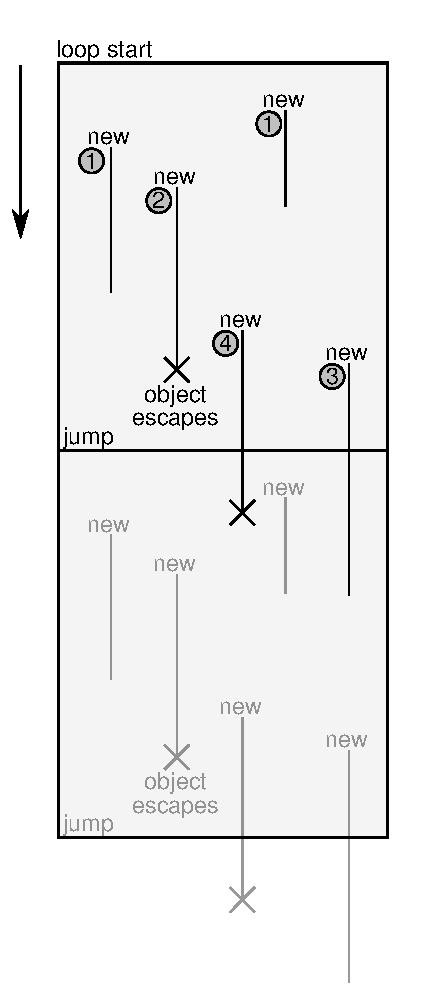
\includegraphics[scale=0.6]{figures/obj-lifetime.pdf}
\end{center}

\caption{Object Lifetimes in a Trace}
\label{fig:lifetimes}
\end{figure}

Figure~\ref{fig:lifetimes} shows a trace before optimization, together with the
lifetime of various kinds of objects created in the trace. It is executed from
top to bottom. At the bottom, a jump is used to execute the same loop another
time (for clarity, the figure shows two iterations of the loop). The loop is
executed until one of the guards in the trace fails, and the execution is
aborted and interpretation resumes.

Some of the operations within this trace are \lstinline{new} operations, which each
create a new instance of some class. These instances are used for some time, \eg
by calling methods on them (which are inlined into the trace), reading and
writing their fields. Some of these instances \emph{escape}, which means that
they are stored in some globally accessible place or are passed into a
non-inlined function via a residual call.

Together with the \lstinline{new} operations, the figure shows the lifetimes of the
created objects. The objects that are created within a trace using \lstinline{new}
fall into one of several categories:

\begin{enumerate}
    \item Objects that live for some time, and are then just not
    used any more afterwards.

    \item Objects that live for some time and then escape.

    \item Objects that live for some time, survive across the jump to
    the beginning of the loop, and are then not used any more.

    \item Objects that live for some time, survive across the jump,
    and then escape. To these we also count the objects that live across several
    jumps and then either escape or stop being used.
\end{enumerate}

The objects that are allocated in the example trace in
Figure~\ref{fig:unopt-trace} fall into categories 1 and 3. Objects stored in
$p_{5}$, $p_{6}$, $p_{11}$ are in category 1, objects in $p_{10}$, $p_{15}$ are in
category 3.

The creation of objects in category 1 is removed by the optimization described
in Sections~\ref{sec:statics} and \ref{sec:formal}. Objects in the other
categories are partially optimized by this approach as well.\footnote{We also started to
work on optimizing objects in category 3, which will be the subject of a later
paper.}

\section{Allocation Removal in Traces}
\label{sec:statics}

The main insight to improve the code shown in Section~\ref{sub:example} is that objects
in category 1 do not survive very long -- they are used only inside the loop and
there is no other outside reference to them. The optimizer identifies objects in
category 1 and removes the allocation of these objects, and all operations
manipulating them.

This is a process that is usually called \emph{escape analysis}
\cite{goldberg_higher_1990}. In this paper we will perform escape analysis by
using partial evaluation. The use of partial evaluation is a bit peculiar in
that it receives no static input arguments for the trace, but it is only used to
optimize operations within the trace. This section will give an informal account
of this process by examining the example trace in Figure~\ref{fig:unopt-trace}.
The final trace after optimization can be seen in Figure~\ref{fig:step1} (the
line numbers are the lines of the unoptimized trace where the operation comes
from).

To optimize the trace, it is traversed from beginning to end and an output trace
is produced at the same time. Every operation in the input trace is either
removed, or put into the output trace. Sometimes new operations need to be
produced as well. The optimizer can only remove operations that manipulate
objects that have been allocated within the trace, while all other operations are copied to the
output trace untouched.

Looking at the example trace of Figure~\ref{fig:unopt-trace}, the operations
in lines 1-9 are manipulating objects which existed before the trace and that
are passed in as arguments: therefore the optimizer just puts them into the
output trace.

The following operations (lines 10-17) are more interesting:
% XXX line numbers

\begin{lstlisting}[mathescape,xleftmargin=20pt]
$p_{5}$ = new(BoxedInteger)
set($p_{5}$, intval, $i_{4}$)
$p_{6}$ = new(BoxedInteger)
set($p_{6}$, intval, -100)
\end{lstlisting}

When the optimizer encounters a \lstinline{new}, it removes it optimistically,
and assumes that the object is in category 1. If later the optimizer finds that the object escapes, it
will be allocated at that point. The optimizer needs to keep track
of the state of the object that the operation would have created.
This is done with the help of a \emph{static object}\footnote{Here
``static'' is meant in the sense of partial evaluation, \ie known at partial
evaluation time, not in the sense of ``static allocation'' or ``static
method''.}. The static object describes the shape of the object that would have
been allocated, \ie the type of the object and where the values that would be
stored in the fields of the allocated object come from.

In the snippet above, the two \lstinline{new} operations are removed and two
static objects are constructed. The \lstinline{set} operations manipulate a
static object, therefore they can be removed as well and their effect is
remembered in the static objects.

The static object associated with $p_{5}$ would store the knowledge that it is a
\lstinline{BoxedInteger} whose \lstinline{intval} field contains $i_{4}$; the
one associated with $p_{6}$ would store that it is a \lstinline{BoxedInteger}
whose \lstinline{intval} field contains the constant -100.

The subsequent operations (line 19-29) in Figure~\ref{fig:unopt-trace}, which
use $p_{5}$ and $p_{6}$, can then be optimized using that knowledge:

\begin{lstlisting}[mathescape,xleftmargin=20pt]
guard_class($p_{5}$, BoxedInteger)
# inside BoxedInteger.add
$i_{7}$ = get($p_{5}$, intval)
guard_class($p_{6}$, BoxedInteger)
# inside BoxedInteger.add__int
$i_{8}$ = get($p_{6}$, intval)
$i_{9}$ = int_add($i_{7}$, $i_{8}$)
\end{lstlisting}

The \lstinline{guard_class} operations can be removed, since their argument is a
static object with the matching type \lstinline{BoxedInteger}. The
\lstinline{get} operations can be removed as well, because each of them reads a
field out of a static object. The results of the get operation are replaced with
what the static object stores in these fields: all the occurences of $i_{7}$ and $i_{8}$ in the trace are just
replaced by $i_{4}$ and -100. The only operation put into the optimized trace
is the addition:

\begin{lstlisting}[mathescape,xleftmargin=20pt]
$i_{9}$ = int_add($i_{4}$, -100)
\end{lstlisting}

The rest of the trace from Figure~\ref{fig:unopt-trace} is optimized in a
similar vein. The operations in lines 27-35 produce two more static objects and
are removed. Those in line 36-39 are just put into the output trace because they
manipulate objects that are allocated before the trace. Lines 40-42 are removed
because they operate on a static object. Line 43 is put into the output trace.
Lines 44-46 produce a new static object and are removed, lines 48-51 manipulate
that static object and are removed as well. Lines 52-54 are put into the output
trace.

The last operation (line 55) is an interesting case. It is the \lstinline{jump}
operation that passes control back to the beginning of the trace. The two
arguments to this operation are at this point static objects. However, because
they passed into the next iteration of the loop they live longer than the trace
and therefore cannot remain static. They need to be turned into a dynamic
(runtime) object before the actual \lstinline{jump} operation. This process of
turning a static object into a dynamic one is called \emph{lifting}.

Lifting a static object puts \lstinline{new} and \lstinline{set} operations into
the output trace. Those operations produce an object at runtime that has the
same shape that the static object describes. This process is a bit delicate,
because the static objects could form an arbitrary graph structure. In our
example is is simple, though:

\begin{lstlisting}[mathescape,xleftmargin=20pt]
$p_{15}$ = new(BoxedInteger)
set($p_{15}$, intval, $i_{14}$)
$p_{10}$ = new(BoxedInteger)
set($p_{10}$, intval, $i_{9}$)
jump($p_{15}$, $p_{10}$)
\end{lstlisting}


Observe how the operations for creating these two instances have been moved to a
later point in the trace. This is worthwhile even though the objects have to be
allocated in the end because some \lstinline{get} operations and
\lstinline{guard_class} operations on the lifted static objects could be
removed.

A bit more generally, lifting needs to occur if a static object is used in any
operation apart from \lstinline{get}, \lstinline{set}, and \lstinline{guard}.
It also needs to occur if \lstinline{set} is used to store a static object into
a non-static one.

The final optimized trace of the example can be seen in Figure~\ref{fig:step1}.
The optimized trace contains only two allocations, instead of the original five,
and only three \lstinline{guard_class} operations, from the original seven.

\begin{figure}
\begin{lstlisting}[mathescape,numbers=right,escapechar=|,numberstyle = \tiny,numbersep=0pt, numberblanklines=false]
# arguments to the trace: $p_{0}$, $p_{1}$ |\setcounter{lstnumber}{2}|
guard_class($p_1$, BoxedInteger)           |\setcounter{lstnumber}{4}|
$i_2$ = get($p_1$, intval)
guard_class($p_0$, BoxedInteger)           |\setcounter{lstnumber}{7}|
$i_3$ = get($p_0$, intval)
$i_4$ = int_add($i_2$, $i_3$)              |\setcounter{lstnumber}{25}|
$i_9$ = int_add($i_4$, -100)               |\setcounter{lstnumber}{35}|

guard_class($p_0$, BoxedInteger)           |\setcounter{lstnumber}{38}|
$i_{12}$ = get($p_0$, intval)              |\setcounter{lstnumber}{42}|
$i_{14}$ = int_add($i_{12}$, -1)           |\setcounter{lstnumber}{50}|

$i_{17}$ = int_gt($i_{14}$, 0)             |\setcounter{lstnumber}{53}|
guard_true($i_{17}$)                       |\setcounter{lstnumber}{42}|

$p_{15}$ = new(BoxedInteger)               |\setcounter{lstnumber}{45}|
set($p_{15}$, intval, $i_{14}$)            |\setcounter{lstnumber}{26}|
$p_{10}$ = new(BoxedInteger)               |\setcounter{lstnumber}{28}|
set($p_{10}$, intval, $i_9$)               |\setcounter{lstnumber}{53}|

jump($p_{15}$, $p_{10}$)
\end{lstlisting}

\caption{Resulting Trace After Allocation Removal}
\label{fig:step1}
\end{figure}


\section{Formal Description of the Algorithm}
\label{sec:formal}


\begin{figure*}
\begin{center}
\begin{tabular}{lcccc}
\emph{new} & ${\displaystyle \frac{l\,\mathrm{fresh}}{v=\mathtt{new}(T),E,H\overset{\mathrm{run}}{\Longrightarrow}E\left[v\mapsto l\right],H\left[l\mapsto\left(T,\mathrm{null},\mathrm{null}\right)\right]}}$ & ~~~ & \emph{guard} & ${\displaystyle \frac{\mathrm{type}(H(E(v))=T}{\mathtt{guard\_class}(v,T),E,H\overset{\mathrm{run}}{\Longrightarrow}E,H}}$\tabularnewline[3em]
\emph{get} & ${\displaystyle \frac{\,}{u=\mathtt{get}(v,F),E,H\overset{\mathrm{run}}{\Longrightarrow}E\left[u\mapsto H\left(E\left(v\right)\right)_{F}\right],H}}$ & ~~~ &  & ${\displaystyle \frac{\mathrm{type}(H(E(v))\neq T}{\mathtt{guard\_class}(v,T),E,H\overset{\mathrm{run}}{\Longrightarrow}\bot,\bot}}$\tabularnewline[3em]
\emph{set} & ${\displaystyle \frac{\,}{\mathtt{set}\left(v,F,u\right),E,H\overset{\mathrm{run}}{\Longrightarrow}E,H\left[E\left(v\right)\mapsto\left(H\left(E\left(v\right)\right)!_{F}E(u)\right)\right]}}$ & ~~~ &  & \tabularnewline[4em]
\end{tabular}
\end{center}

\begin{minipage}[b]{7 cm}
\emph{Object Domains:}
$$\setlength\arraycolsep{0.1em}
 \begin{array}{rcll}
    u,v & \in & V & \mathrm{\ variables\ in\ trace}\\
    T & \in & \mathfrak{T} & \mathrm{\ runtime\ types}\\
    F & \in & \left\{ L,R\right\} & \mathrm{\ fields\ of\ objects}\\
    l & \in & L & \mathrm{\ locations\ on\ heap}
 \end{array}
$$
\end{minipage}
\begin{minipage}[b]{5 cm}
\emph{Semantic Values:}
$$\setlength\arraycolsep{0.1em}
 \begin{array}{rcll}
    E & \in & V\rightharpoonup L & \mathrm{\ Environment}\\
    H & \in & L\rightharpoonup\mathfrak{T}\times(L\cup \{ \mathrm{null} \})\times (L\cup \{ \mathrm{null}\} ) & \mathrm{\ Heap}\\
    \\
    \\
 \end{array}
$$
\end{minipage}
\caption{The Operational Semantics of Simplified Traces}
\label{fig:semantics}
\end{figure*}

In this section we want to give a formal description of the semantics of the
traces and of the optimizer and liken the optimization to partial evaluation.
We focus on the operations for manipulating dynamically allocated objects,
as those are the only ones that are actually optimized. We also consider only
objects with two fields in this section, generalizing to arbitrary many fields
is straightforward.

Traces are lists of operations. The operations considered here are
\lstinline{new}, \lstinline{get}, \lstinline{set} and \lstinline{guard_class}.
The values of all
variables are locations (\ie pointers). Locations are mapped to objects, which
are represented by triples of a type $T$, and two locations that represent the
fields of the object. When a new object is created, the fields are initialized
to null, but we require that they are initialized to a real
location before being read, otherwise the trace is malformed (this condition is
guaranteed by how the traces are generated in PyPy).

We use some abbreviations when dealing with object triples. To read the type of
an object, $\mathrm{type}((T,l_1,l_2))=T$ is used. Reading a field $F$ from an
object is written $(T,l_1,l_2)_F$ which either returns $l_1$ if $F=L$ or $l_2$
if $F=R$. To set field $F$ to a new location $l$, we use the notation
$(T,l_1,l_2)!_Fl$, which yields a new triple $(T,l,l_2)$ if $F=L$ or a new
triple $(T,l_1,l)$ if $F=R$.

Figure~\ref{fig:semantics} shows the operational semantics for traces. The
interpreter formalized there executes one operation at a time. Its state is
represented by an environment $E$ and a heap $H$, which may be changed by the
execution of an operation. The environment is a partial function from variables
to locations and the heap is a partial function from locations to objects. Note
that a variable can never be null in the environment, otherwise the trace would have
been malformed. The environment could not directly map variables to objects,
because several variables can point to the \emph{same} object, because of aliasing. 

We use the following notation for updating partial functions:
$E[v\mapsto l]$ denotes the environment which is just like $E$, but maps $v$ to
$l$.

The \lstinline{new} operation creates a new object $(T,\mathrm{null},\mathrm{null})$ on the
heap under a fresh location $l$ and adds the result variable to the environment,
mapping it to the new location $l$.

The \lstinline{get} operation reads a field $F$ out of an object, and adds the result
variable to the environment, mapping it to the read location. The heap is
unchanged.

The \lstinline{set} operation changes field $F$ of an object stored at the location that
variable $v$ maps to. The new value of the field is the location in variable
$u$. The environment is unchanged.

The \lstinline{guard_class} operation is used to check whether the object stored at the location
that variable $v$ maps to is of type $T$. If that is the case, then execution
continues without changing heap and environment. Otherwise, execution is
stopped.

\subsection{Optimizing Traces}
\label{sub:formalopt}



\begin{figure*}
\begin{center}
\begin{tabular}{lc}
\emph{new} & ${\displaystyle \frac{v^{*}\,\mathrm{fresh}}{v=\mathtt{new}(T),E,S\overset{\mathrm{opt}}{\Longrightarrow}\left\langle \,\right\rangle ,E\left[v\mapsto v^{*}\right],S\left[v^{*}\mapsto\left(T,\mathrm{null,null}\right)\right]}}$\tabularnewline[3em]
\emph{get} & ${\displaystyle \frac{E(v)\in\mathrm{dom}(S)}{u=\mathtt{get}(v,F),E,S\overset{\mathrm{opt}}{\Longrightarrow}\left\langle \,\right\rangle ,E\left[u\mapsto S(E(v))_{F}\right],S}}$\tabularnewline[3em]
 & ${\displaystyle \frac{E(v)\notin\mathrm{dom}(S),\,\,\, u^{*}\,\mathrm{fresh}}{u=\mathtt{get}(v,F),E,S\overset{\mathrm{opt}}{\Longrightarrow}\left\langle u^{*}=\mathtt{get}(E(v),F)\right\rangle ,E\left[u\mapsto u^{*}\right],S}}$\tabularnewline[3em]
\emph{set} & ${\displaystyle \frac{E(v)\in\mathrm{dom}(S)}{\mathtt{set}\left(v,F,u\right),E,S\overset{\mathrm{opt}}{\Longrightarrow}\left\langle \,\right\rangle ,E,S\left[E\left(v\right)\mapsto\left(S(E(v))!_{F}E(u)\right)\right]}}$\tabularnewline[3em]
 & ${\displaystyle \frac{E(v)\notin\mathrm{dom}\left(S\right),\,\left(E(v),S\right)\overset{\mathrm{lift}}{\Longrightarrow}\left(\mathrm{ops},S^{\prime}\right)}{\mathtt{set}\left(v,F,u\right),E,S\overset{\mathrm{opt}}{\Longrightarrow}\mathrm{ops}::\left\langle \mathtt{set}\left(E(v),F,E(u)\right)\right\rangle ,E,S^{\prime}}}$\tabularnewline[3em]
\emph{guard} & ${\displaystyle \frac{E(v)\in\mathrm{dom}(S),\,\mathrm{type}(S(E(v)))=T}{\mathtt{guard\_class}(v,T),E,S\overset{\mathrm{opt}}{\Longrightarrow}\left\langle \,\right\rangle ,E,S}}$\tabularnewline[3em]
 & ${\displaystyle \frac{E(v)\notin\mathrm{dom}(S)\vee\mathrm{type}(S(E(v)))\neq T,\,\left(E(v),S\right)\overset{\mathrm{lift}}{\Longrightarrow}\left(\mathrm{ops},S^{\prime}\right)}{\mathtt{guard\_class}(v,T),E,S\overset{\mathrm{opt}}{\Longrightarrow}\mathrm{ops}::\left\langle \mathtt{guard\_class}(E\left(v\right),T)\right\rangle ,E,S^{\prime}}}$\tabularnewline[3em]
\emph{lifting} & ${\displaystyle \frac{v^{*}\notin\mathrm{dom}(S)}{v^{*},S\overset{\mathrm{lift}}{\Longrightarrow}\left\langle \,\right\rangle ,S}}$\tabularnewline[3em]
 & ${\displaystyle \frac{v^{*}\in\mathrm{dom}(S),\,\left(v^{*},S\right)\overset{\mathrm{liftfields}}{=\!=\!\Longrightarrow}\left(\mathrm{ops},S^{\prime}\right)}{v^{*},S\overset{\mathrm{lift}}{\Longrightarrow}\left\langle v^{*}=\mathtt{new}\left(T\right)\right\rangle ::ops,S^{\prime}}}$\tabularnewline[3em]
 & ${\displaystyle \frac{\left(S\left(v^{*}\right)_{L},S\setminus\left\{ v^{*}\mapsto S\left(v^{*}\right)\right\} \right)\overset{\mathrm{lift}}{\Longrightarrow}\left(\mathrm{ops}_{L},S^{\prime}\right),\,\left(S\left(v^{*}\right)_{R},S^{\prime}\right)\overset{\mathrm{lift}}{\Longrightarrow}\left(\mathrm{ops}_{R},S^{\prime\prime}\right)}{v^{*},S\overset{\mathrm{liftfields}}{=\!=\!\Longrightarrow}\mathrm{ops}_{L}::ops_{R}::\left\langle \mathtt{set}\left(v^{*},L,S\left(v^{*}\right)_{L}\right),\,\mathtt{set}\left(v^{*},R,S\left(v^{*}\right)_{R}\right)\right\rangle ,S^{\prime}}}$\tabularnewline[3em]
\end{tabular}
\end{center}

\begin{minipage}[b]{7 cm}
\emph{Object Domains:}
$$\setlength\arraycolsep{0.1em}
 \begin{array}{rcll}
    u,v & \in & V & \mathrm{\ variables\ in\ trace}\\
    u^*,v^* & \in & V^* & \mathrm{\ variables\ in\ optimized\ trace}\\
    T & \in & \mathfrak{T} & \mathrm{\ runtime\ types}\\
    F & \in & \left\{ L,R\right\} & \mathrm{\ fields\ of\ objects}\\
 \end{array}
$$
\end{minipage}
\begin{minipage}[b]{5 cm}
\emph{Semantic Values:}
$$\setlength\arraycolsep{0.1em}
 \begin{array}{rcll}
    E & \in & V\rightharpoonup V^* & \mathrm{\ Environment}\\
    S & \in & V^*\rightharpoonup\mathfrak{T}\times(V^*\cup \{ \mathrm{null} \})\times (V^*\cup \{ \mathrm{null}\} ) & \mathrm{\ Static\ Heap}\\
    \\
    \\
 \end{array}
$$
\end{minipage}
\caption{Optimization Rules}
\label{fig:optimization}
\end{figure*}

To optimize the simple traces of the last section, we use online partial
evaluation. The partial evaluator optimizes one operation of a trace at a
time. Every operation in the unoptimized trace is replaced by a list of
operations in the optimized trace. This list is empty if the operation can be
optimized away. The optimization rules can be seen in
Figure~\ref{fig:optimization}. Lists are written using angular brackets $<...>$,
list concatenation is expressed using two colons: $l_1::l_2$.

XXX input/output of optimizer

The state of the optimizer is stored in an environment $E$ and a \emph{static
heap} $S$. The environment is a partial function from variables in the
unoptimized trace $V$ to variables in the optimized trace $V^*$ (which are
themselves written with a
$\ ^*$ for clarity). The reason for introducing new variables in the optimized
trace is that several variables that appear in the unoptimized trace can turn
into the same variables in the optimized trace. The environment of the
optimizer serves a function similar to that of the environment in the
semantics: to express sharing.

The static heap is a partial function from $V^*$ into the
set of static objects, which are triples of a type and two elements of $V^*$.
The object referenced by a variable $v^*$ is static, if $v^*$ is in the domain
of the static heap $S$. The object $S(v^*)$ describes
what is statically known about the object, \ie its type and its fields. The
fields of objects in the static heap are also elements of $V^*$ (or null, for
short periods of time).

When the optimizer sees a \lstinline{new} operation, it optimistically removes it and
assumes that the resulting object can stay static. The optimization for all
further operations is split into two cases. One case is for when the
involved variables are in the static heap, which means that the operation can be
performed at optimization time and can be removed from the trace. These rules mirror
the execution semantics closely. The other case is for when not enough is known about
the variables, and the operation has to be residualized.

If the argument $v$ of a \lstinline{get} operation is mapped to something in the static
heap, the \lstinline{get} can be performed at optimization time. Otherwise, the \lstinline{get}
operation needs to be residualized.

If the first argument $v$ to a \lstinline{set} operation is mapped to something in the
static heap, then the \lstinline{set} can be performed at optimization time
(which updates the static heap). Otherwise the \lstinline{set} operation needs
to be residualized. This needs to be
done carefully, because the new value for the field, from the variable $u$,
could itself be static, in which case it needs to be lifted first.

If a \lstinline{guard_class} is performed on a variable that is in the static heap, the type check
can be performed at optimization time, which means the operation can be removed
if the types match. If the type check fails statically or if the object is not
in the static heap, the \lstinline{guard_class} is residualized. This also needs to
lift the variable on which the \lstinline{guard_class} is performed.

Lifting takes a variable and turns it into a dynamic variable. If the variable
is already dynamic, nothing needs to be done. If it is in the static heap,
operations are emitted that construct an object with the shape described
there, and the variable is removed from the static heap.

Lifting a static object needs to recursively lift its fields. Some care needs to
be taken when lifting a static object, because the structures described by the
static heap can be cyclic. To make sure that the same static object is not lifted
twice, the \lstinline{liftfield} operation removes it from the static heap \emph{before}
recursively lifting its fields.

As an example for lifting, consider the static heap $$\{v^* \mapsto (T_1, w^*,
v^*), w^* \mapsto (T_2, u^*, u^*)\}$$ which contains two static objects. If $v^*$
needs to be lifted, the following residual operations are produced:

\begin{lstlisting}[mathescape,xleftmargin=20pt]
$v^*$ = new($T_1$)
$w^*$ = new($T_2$)
set($w^*$, $L$, $u^*$)
set($w^*$, $R$, $u^*$)
set($v^*$, $L$, $w^*$)
set($v^*$, $R$, $v^*$)
\end{lstlisting}

After the lifting the static heap is the empty set, because both static objects
were lifted.
If we had lifted $w^*$ instead of $v^*$, then the following operations would
have been produced:

\begin{lstlisting}[mathescape,xleftmargin=20pt]
$w^*$ = new($T_2$)
set($w^*$, $L$, $u^*$)
set($w^*$, $R$, $u^*$)
\end{lstlisting}

In this case, the static heap afterwards would be:
$$\{v^* \mapsto (T_1, w^*, v^*)\}$$



% subsection Optimizing Traces (end)

\subsection{Analysis of the Algorithm}
\label{sub:analysis}

While we do not offer a formal proof of it, it should be relatively clear
that the algorithm presented above is sound: it works by delaying (and
often completely removing) some operations.  The algorithm runs in a
single pass over the list of operations.  We can check that although
recursively lifting a static object is not a constant-time operation,
the algorithm only takes a total time linear in the length of the trace.
The algorithm itself is not particularly complex; our focus is
rather that \emph{in the context of tracing JITs} it is possible to find a
simple enough algorithm that performs well.

Note in particular that objects in category 1 (\ie those that do
not escape) are completely removed; moreover, objects in category 2
(\ie escaping) are still partially optimized: all the operations in between the
creation of the object and the point where it escapes that involve the object
are removed. Objects in category 3 and 4 are also partially optimized, their
allocation is delayed till the end of the trace.

The optimization is particularly effective for chains of operations.
For example, it is typical for an interpreter to generate sequences of
writes-followed-by-reads, where one interpreted opcode writes to some
object's field and the next interpreted opcode reads it back, possibly
dispatching on the type of the object created just before.  A typical example
would be a chain of arithmetic operations.

% subsection Analysis of the Algorithm (end)

% section Formal Description of the Algorithm (end)

%___________________________________________________________________________

% section Escape Analysis in a Tracing JIT (end)

\section{Implementation and Evaluation}
\label{sec:Evaluation}

The allocation removal techniques described in this paper were implemented in
the optimizer of PyPy's tracing JIT. The optimization is independent of which
interpreter a JIT is generated for. There are some practical issues beyond the
techniques described in this paper. The actual implementation needs to deal with
more operations than described in Section~\ref{sec:formal}, \eg to
also support static arrays in addition to static objects. The implementation of
this optimization is about 400 lines of RPython code.

A further complication is that most interpreters written with PyPy use
heap-allocated frame objects to store local variables. Those severely hinder
the effectiveness of allocation removal, because every time an object is stored
into a local variable, it is stored into the frame-object, which makes it
escape. We implemented a technique to treat such frames objects in a
special way to solve this problem. This is a common approach in VM
implementations \cite{miranda_context_1999,andreas_gal_trace-based_2009}; the
novelty of our approach is that we generalized it enough to be usable for
different interpreters.

To evaluate our allocation removal algorithm, we look at the effectiveness when
used in the generated tracing JIT of PyPy's Python interpreter. This interpreter
is a full implementation of Python 2.5 language semantics and is about 30'000
lines of code.

The
benchmarks we used are small-to-medium Python programs, some synthetic
benchmarks, some real applications.\footnote{All the source code of the
benchmarks can be found at \texttt{http://codespeak.net/svn/pypy/benchmarks/}.
There is also a website that monitors PyPy's performance nightly at
\texttt{http://speed.pypy.org/}.}

Some of them are from the Computer Language Benchmark
Game\footnote{\texttt{http://shootout.alioth.debian.org/}}: \textbf{fannkuch},
\textbf{nbody}, \textbf{meteor-contest}, \textbf{spectral-norm}.

Furthermore there are the following benchmarks:
\begin{itemize}
    \item \textbf{crypto\_pyaes}: An AES implementation.
    \item \textbf{django}: The templating engine of the Django web
    framework\footnote{\texttt{http://www.djangoproject.com/}}.
    \item \textbf{go}: A Monte-Carlo Go
    AI\footnote{\texttt{http://shed-skin.blogspot.com/2009/07/ disco-elegant-python-go-player.html}}.
    \item \textbf{html5lib}: An HTML5 parser.
    \item \textbf{pyflate-fast}: A BZ2 decoder.
    \item \textbf{raytrace-simple}: A ray tracer.
    \item \textbf{richards}: The Richards benchmark.
    \item \textbf{spambayes}: A Bayesian spam filter\footnote{\texttt{http://spambayes.sourceforge.net/}}.
    \item \textbf{telco}: A Python version of the Telco decimal
    benchmark\footnote{\texttt{http://speleotrove.com/decimal/telco.html}},
    using a pure Python decimal floating point implementation.
    \item \textbf{twisted\_names}: A DNS server benchmark using the Twisted networking
    framework\footnote{\texttt{http://twistedmatrix.com/}}.
\end{itemize}


We evaluate the allocation removal algorithm along two lines: first we want to
know how many allocations could be optimized away. On the other hand, we want
to know how much the run times of the benchmarks is improved.

The benchmarks were run on an otherwise idle Intel Core2 Duo P8400 processor
with 2.26 GHz and 3072 KB of cache on a machine with 3GB RAM running Linux
2.6.35. We compared the performance of various Python implementations on the
benchmarks. As a baseline, we used the standard Python implementation in C,
CPython 2.6.6\footnote{\texttt{http://python.org}}, which uses a bytecode-based
interpreter. Furthermore we compared against
Psyco\cite{rigo_representation-based_2004} 1.6,
an extension to CPython which is a
just-in-time compiler that produces machine code at run-time. It is not based
on traces. Finally, we used two versions of PyPy's Python interpreter (revision
77823 of SVN trunk\footnote{\texttt{http://codespeak.net/svn/pypy/trunk}}): one
including the JIT but not optimizing the traces, and one using the allocation
removal optimizations (as well as some minor other optimizations, such as
constant folding).

As the first step, we counted the occurring operations in all generated traces
before and after the optimization phase for all benchmarks. The resulting
numbers can be
seen in Figure~\ref{fig:numops}. The optimization removes between 4\% and 90\%
and of allocation operations in the traces of the benchmarks.
All benchmarks taken together, the optimization removes 70\% percent of
allocation operations. The numbers look similar for reading and writing of
attributes. There are even more \lstinline{guard} operations that are removed,
however there is an additional optimization that removes guards, so not all the
removed guards are an effect of the optimization described here (for technical
reasons, it would be very hard to separate the two effects).

\begin{figure*}
{\small
\begin{center}
\begin{tabular}{|l||r|rr|rr|rr|rr|}
\hline
	&num loops      &new    &removed        &get/set        &removed &guard &removed        &all ops        &removed\\
\hline
crypto\_pyaes	&78	&3088	&50\%	&57148	&25\%	&9055	&95\%	&137189	&80\%\\
django	&51	&673	&54\%	&19318	&18\%	&3876	&93\%	&55682	&85\%\\
fannkuch	&43	&171	&49\%	&886	&63\%	&1159	&81\%	&4935	&45\%\\
go	&517	&12234	&76\%	&200842	&21\%	&53138	&90\%	&568542	&84\%\\
html5lib	&498	&14432	&68\%	&503390	&11\%	&71592	&94\%	&1405780	&91\%\\
meteor-contest	&59	&277	&36\%	&4402	&31\%	&1078	&83\%	&12862	&68\%\\
nbody	&13	&96	&38\%	&443	&69\%	&449	&78\%	&2107	&38\%\\
pyflate-fast	&162	&2278	&55\%	&39126	&20\%	&8194	&92\%	&112857	&80\%\\
raytrace-simple	&120	&3118	&59\%	&91982	&15\%	&13572	&95\%	&247436	&89\%\\
richards	&87	&844	&4\%	&49875	&22\%	&4130	&91\%	&133898	&83\%\\
spambayes	&314	&5608	&79\%	&117002	&11\%	&25313	&94\%	&324125	&90\%\\
spectral-norm	&38	&360	&64\%	&5553	&20\%	&1122	&92\%	&11878	&77\%\\
telco	&46	&1257	&90\%	&37470	&3\%	&6644	&99\%	&98590	&97\%\\
twisted-names	&214	&5273	&84\%	&100010	&10\%	&23247	&96\%	&279667	&92\%\\
\hline
total	&2240	&49709	&70\%	&1227447	&14\%	&222569	&93\%	&3395548	&89\%\\
\hline
\end{tabular}
\end{center}
}
\caption{Number of Operations and Percentage Removed By Optimization}
\label{fig:numops}
\end{figure*}

In addition to the count of operations we also performed time measurements.
All benchmarks were run 50 times in the same process, to give the JIT time to produce machine
code. The arithmetic mean of the times of the last 30 runs were used as the
result. The errors were computed using a confidence interval with a 95\%
confidence level \cite{georges_statistically_2007}. The results are reported in
Figure~\ref{fig:times}. In addition to the run times the table also reports the
speedup that PyPy achieves when the optimization is turned on. XXX sounds sucky

With the optimization turned on, PyPy's Python interpreter outperforms CPython
in all benchmarks except spambayes (which heavily relies on regular expression
performance and thus is not helped much by our Python JIT) and meteor-contest.
All benchmarks are improved by the allocation removal optimization, by at least
20\% and by as much as a factor of 6.95.

Psyco is able to outperform PyPy's JIT in five out of 14 benchmarks. We hope to
overtake Psyco (which is no longer being actively developped) by adding some
further optimizations.

\begin{figure*}
{\small
\begin{center}
\begin{tabular}{|l||r|r||r|r||r|r||r|r|}
\hline
	&CPython [ms]	& $\times$ &Psyco [ms]	& $\times$ &PyPy w/o optim. [ms] & $\times$ &PyPy w/ optim. [ms]& $\times$ \\
\hline
crypto\_pyaes	&2757.80 $\pm$ 0.98	&10.33	&67.90 $\pm$ 0.47	&0.25	&1652.00 $\pm$ 4.00	&6.19	&266.86 $\pm$ 5.94	&1.00\\
django	&993.19 $\pm$ 0.50	&3.83	&913.51 $\pm$ 4.22	&3.52	&694.73 $\pm$ 2.86	&2.68	&259.53 $\pm$ 1.79	&1.00\\
fannkuch	&1987.22 $\pm$ 2.02	&4.26	&944.44 $\pm$ 0.61	&2.02	&566.99 $\pm$ 1.06	&1.21	&466.87 $\pm$ 1.85	&1.00\\
go	&947.21 $\pm$ 1.58	&3.00	&445.96 $\pm$ 0.68	&1.41	&2197.71 $\pm$ 25.21	&6.95	&316.15 $\pm$ 9.33	&1.00\\
html5lib	&13987.12 $\pm$ 19.51	&1.39	&17398.25 $\pm$ 36.50	&1.72	&27194.45 $\pm$ 46.62	&2.69	&10092.19 $\pm$ 23.50	&1.00\\
meteor-contest	&346.98 $\pm$ 0.35	&0.88	&215.66 $\pm$ 0.23	&0.55	&433.04 $\pm$ 1.45	&1.10	&392.85 $\pm$ 0.87	&1.00\\
nbody\_modified	&637.90 $\pm$ 1.82	&6.14	&256.78 $\pm$ 0.18	&2.47	&135.55 $\pm$ 0.33	&1.30	&103.93 $\pm$ 0.25	&1.00\\
pyflate-fast	&3169.35 $\pm$ 1.89	&1.74	&1278.16 $\pm$ 3.13	&0.70	&3285.89 $\pm$ 8.51	&1.80	&1822.36 $\pm$ 11.52	&1.00\\
raytrace-simple	&2744.60 $\pm$ 51.72	&4.24	&1072.66 $\pm$ 1.08	&1.66	&2778.27 $\pm$ 15.13	&4.29	&647.24 $\pm$ 5.44	&1.00\\
richards	&354.06 $\pm$ 1.00	&4.01	&63.48 $\pm$ 0.15	&0.72	&383.93 $\pm$ 3.28	&4.35	&88.32 $\pm$ 0.91	&1.00\\
spambayes	&299.16 $\pm$ 0.35	&0.75	&338.68 $\pm$ 3.14	&0.85	&580.90 $\pm$ 24.68	&1.46	&397.37 $\pm$ 10.60	&1.00\\
spectral-norm	&478.63 $\pm$ 0.80	&4.27	&139.83 $\pm$ 1.54	&1.25	&353.51 $\pm$ 1.39	&3.15	&112.10 $\pm$ 1.17	&1.00\\
telco	&1207.67 $\pm$ 2.03	&2.44	&730.00 $\pm$ 2.66	&1.47	&1296.08 $\pm$ 4.37	&2.62	&495.23 $\pm$ 2.14	&1.00\\
twisted\_names	&9.58 $\pm$ 0.01	&1.34	&10.43 $\pm$ 0.01	&1.46	&17.99 $\pm$ 0.27	&2.52	&7.13 $\pm$ 0.09	&1.00\\
\hline
\end{tabular}
\end{center}
}
\caption{Benchmark Times in Milliseconds, Together With Factor Over PyPy With Optimizations}
\label{fig:times}
\end{figure*}

\section{Related Work}
\label{sec:related}

There exists a large number of works on escape analysis, which is a program
analysis that tries to find an upper bound for the lifetime of objects allocated
at specific program points
\cite{goldberg_higher_1990,park_escape_1992,choi_escape_1999,bruno_blanchet_escape_2003}.
This information can then be used to decide that certain objects can be
allocated on the stack, because their lifetime does not exceed that of the stack
frame it is allocated in. The difference to our work is that escape analysis is
split into an analysis and an optimization phase. The analysis can be a lot more
complex than our simple one-pass optimization. Also, stack-allocation reduces
garbage-collection pressure but does not optimize away the actual accesses to
the stack-allocated object. In our case, an object is not needed at all any
more.

Chang \etal describe a tracing JIT for JavaScript running on top of a JVM
\cite{mason_chang_efficient_2007}. They mention in passing an approach to
allocation removal that moves the allocation of an object of type 1 out of the
loop to only allocate it once, instead of every iteration. No details are given
for this optimization. The fact that the object is still allocated and needs to
be written to means that only the allocations are optimized away, but not the
reads and writes out of/into the object.

SPUR, a tracing JIT for C\# seems to be able to remove allocations in a similar
way to the approach described here, as hinted at in the technical report
\cite{michael_bebenita_spur:_2010}. However, no details for the approach and its
implementation are given.

Psyco \cite{rigo_representation-based_2004} is a (non-tracing) JIT for Python
that implements a more ad-hoc version of the allocation removal described here.
Our static objects could be related to what are called \emph{virtual} objects
in Psyco.  It is a hand-written extension module for CPython. Historically,
PyPy's JIT can be seen as some successor of Psyco for a general context (one of
the authors of this paper is the author of Psyco).

The original SELF JIT compiler \cite{chambers_efficient_1989} used an algorithm for
forward-propagating the types of variables as part of its optimizations. This
makes it possible to remove all type checks on a variable but the first one.
The optimization does not deal with removing the full object, if it is
short-lived, but the type check removals are similar to what our optimization
achieves.

Partially known data structures are built directly into Prolog (via unbound
logic variables) and thus the treatment of partially static data structures
was part of partial evaluation of Prolog programs from the early stages
\cite{lloyd_partial_1991}. One effect of unfolding in Prolog is that terms that
are constructed and immediately matched again, completely disappear in the
residual program. This is similar to what our optimization does for an
imperative language.
In functional programming this idea was introduced as
 constructor specialisation by Mogensen \cite{Mogensen:PEPM93}.

%xxx:
%partially static data structures: kenichi asai's thesis?

%xxx: 
%Other related work is compile-time garbage collection \cite{mazur_practical_2001}, which
%tries to ....;
%  separation logic
  %; John Hughes: type specialization

\section{Conclusion and Future Work}
\label{sec:conclusion}

In this paper, we used an approach based on online partial evaluation
to optimize away allocations and type guards in the traces of a
tracing JIT.  In this context a simple approach based on partial evaluation
gives good results.  This is due to the fact that the tracing JIT
itself is responsible for all control issues, which are usually the
hardest part of partial evaluation: the tracing JIT selects the parts
of the program that are worthwhile to optimize, and extracts linear
paths through them, inlining functions as necessary.  What is left to
optimize are only those linear paths.

We expect a similar result for other optimizations that usually require
a complex analysis phase and are thus normally too slow to use at
runtime.  A tracing JIT selects interesting linear paths by itself;
therefore, a naive version of many optimizations on such paths should
give mostly the same results.  For example, we experimented with (and
plan to write about) store-load propagation with a very simple alias
analysis.


\section*{Acknowledgements}

The authors would like to thank Stefan Hallerstede, David Schneider and Thomas
Stiehl for fruitful discussions and detailed feedback during the writing of the
paper.

\bibliographystyle{abbrv}
\bibliography{paper}

\end{document}
